\documentclass[a4paper]{article}

\usepackage{graphicx}
\usepackage{amsmath,amssymb}
\usepackage{minted}
\usepackage{multirow}
\usepackage{float}
\usepackage{todonotes}
\usepackage{forest}
\usepackage{xstring}
\usepackage{xcolor}
\usepackage[most]{tcolorbox}
\usepackage{xparse}
\usepackage{natbib}

\usetikzlibrary{graphs,graphdrawing}
\usegdlibrary{layered}

% for external graphviz
\input{/home/donkarlo/Dropbox/repo/nd_language_ai_project/src/nd_language_ai/formal/computer/programming/tex/latex/code_clips/external_graphviz.tex}

% for tags
\input{/home/donkarlo/Dropbox/repo/nd_language_ai_project/src/nd_language_ai/formal/computer/programming/tex/latex/part/control_sequence/kind/semtag/semtag.tex}

% for links
\input{/home/donkarlo/Dropbox/repo/nd_language_ai_project/src/nd_language_ai/formal/computer/programming/tex/latex/code_clips/seehere.tex}

\title{Language}
\date{}
\author{Mohammad Rahmani}

\begin{document}

   \maketitle

   \label{language}
   The role of language here is to provide replaceable components whose meaningfulness can be assessed when they are substituted, thereby providing a measure for anomaly detection. In other words, they tighten the conditions for discrepancy detection.

   Each utterance of a language can be considered a variable-length sequence (rather than a time series, because language components have no time indices unless they are independently specified as members of the sequence) of replaceable components that are themselves composed of other replaceable components. The function of a linguistic system is to assign a probability to each utterance sequence based on the context in which it occurs.

   The system proposed in this research is composed of the architecture shown below.
   \begin{figure}[H]
      \centering
      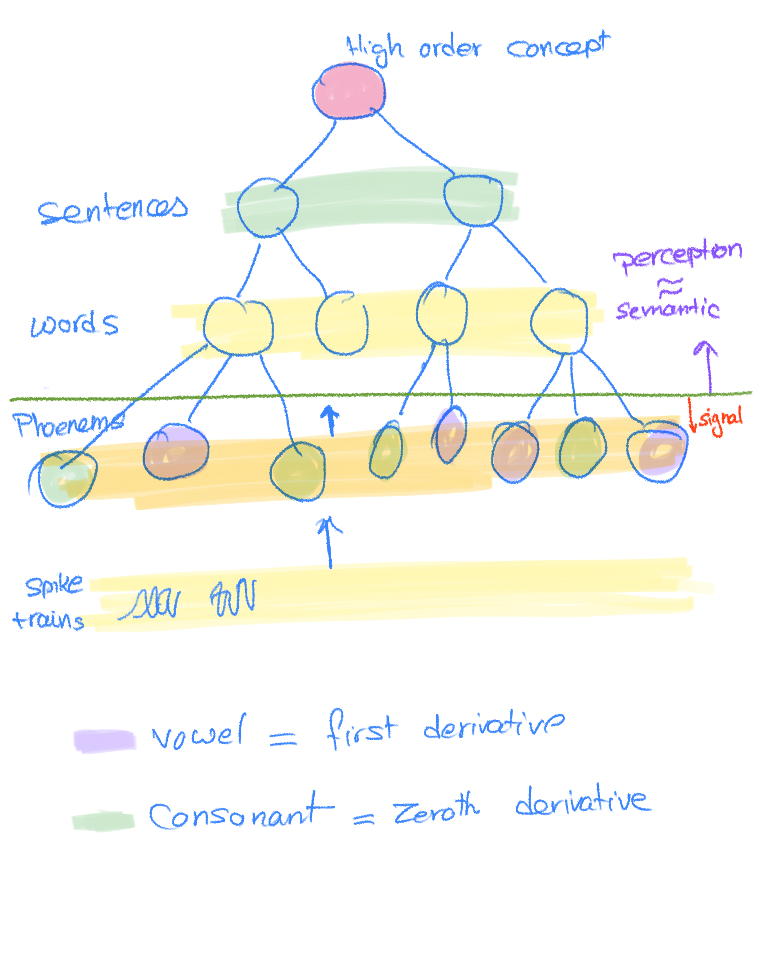
\includegraphics[width=0.9\textwidth]{language_architecture.png}
   \end{figure}

   Language makes it more difficult for the system to classify a course of events as abnormal because it provides a mechanism for replacing and testing different lower-level components to determine the extent to which a confidence interval can be assigned to the given sequence.

   Language is considered in terms of verb--noun pairs, and consonant--vowel pairs are also treated as a noun--verb architecture, even though the human brain ultimately combines them into the same meaning.

   For the sake of simplicity, a neuron is used to represent a language component, although this is not biologically exact and a circuit in the human brain is activated for each word. By language, we mean Ferdinand de Saussure's theory of language, which states that language is formed from the following components.
   \begin{itemize}
      \item \textbf{Syntagmatic axis:} language elements combine in a linear sequence, for example words forming a sentence.
      \item \textbf{Paradigmatic axis:} language elements can replace each other in the same position, changing the meaning or value of the expression.
   \end{itemize}

   Saussure argues that linguistic signs acquire their value through their differences and relations with other signs within the language system \cite{saussure-1966-course-in-general-linguistics}. Lévi-Strauss extends this structural principle to culture and myth, where meaning is often organized through relational structures and binary oppositions \cite{levi-strauss-1955-the-structural-study-of-myth}.
   Test is here

   The method proposed in this paper considers anomaly detection, and at a higher level novelty detection, as part of Saussure's structural view, in which dichotomies such as anomaly versus normality, novelty versus familiarity, and outlier versus inlier are treated as signs used by the agent.

   If the agent can say "I am aware", where "I" is distinguished from "other" and awareness is distinguished from unawareness, then we can say that this agent is aware of its own awareness; in other words, it is a self-aware agent.

   Thus, the main objective of this research is to enable the agent to distinguish between itself and others (the self component of self-awareness) and between novelty and familiarity (the awareness component of self-awareness).

   In other words, the proposed system models a novelty-based component of awareness, particularly the conscious detection of violations of learned global regularities.


   The proposed architecture therefore separates the self-awareness problem into two explicit distinctions:
   \[
   C_{\mathrm{self}} \neq C_{\mathrm{other}}
   \]
   and
   \[
   C_{\mathrm{aware}} \neq C_{\mathrm{unaware}}.
   \]

   The proposition ``I am aware'' can then be interpreted as the combination of a self-representation and a representation of the agent's own awareness state:
   \[
   \text{``I am aware''}
   =
   \text{self-representation}
   +
   \text{representation of awareness}.
   \]

   From a structural perspective, the process can be summarized as
   \[
   \text{sensory data}
   \rightarrow
   \text{distinctions}
   \rightarrow
   \text{categories}
   \rightarrow
   \text{signs}
   \rightarrow
   \text{language}.
   \]


   \begin{itemize}
      \item Each language component, such as a word, is itself represented by a grandmother neuron.
      \item Each component is the result of DBSCAN clustering at the phoneme level and motif discovery from the word level.
   \end{itemize}

   \section{Jargon}
      Examples of words used in the experiments section
      \begin{itemize}
         \item turn from west to east
         \item turn from east to north
         \item turn from north to west
         \item turn from west to south
         \item go straight south
         \item go straight north
         \item go straight west
         \item go straight east
      \end{itemize}


         \bibliographystyle{plainnat}
         \bibliography{/home/donkarlo/Dropbox/repo/nd_shared_research/bibliography/bibliography.bib}

\end{document}
